\begin{definition}
    Inwersja w permutacji $\sigma \in S_n$ to taka para $\sigma(i), \sigma(j)$, że
    \[ i < j, \qquad \sigma(i) > \sigma(j). \]
\end{definition}

\begin{definition}
    Znak permutacji $\sigma$ to
    \[ \eps(\sigma) = (-1)^{[\sigma]}, \]
    gdzie $[\sigma]$ to liczba inwersji w permutacji $\sigma$.
\end{definition}

Jeśli $\eps(\sigma) = 1$, to permutacja $\sigma$ jest \vocab{parzysta}, a jeśli  $\eps(\sigma) = -1$, to jest \vocab{nieparzysta}.

\begin{fact}
    \label{f:sign of transposition}
    Każda transpozycja (zamiana miejscami) dwóch różnych elementów permutacji zmienia jej znak.
\end{fact}
\begin{proof}
    Weźmy permutację
    \[ (\sigma_1, \sigma_2, \ldots, \sigma_i, \ldots, \sigma_j, \ldots, \sigma-{n-1}, \sigma_n). \]
    Zamieniając $\sigma_i$ oraz $\sigma_j$ nie zmieni się liczba inwersji zawierająch elementy $\sigma_k, k \in [1,i)\cup(j,n]$. Nie zmieni się również liczba inwersji zawierających elementy $\sigma_k, k \in (i,j)$ takie, że $\sigma_k$ jest większe lub mniejsze jednocześnie od $\sigma_i$ i $\sigma_j$.

    Dla pozostałych elementów $\sigma_k, k \in (i, j)$ jeśli istnieje inwersja $(\sigma_i, \sigma_k)$ to istnieje również $(\sigma_k, \sigma_j)$, a jeśli istnieje inwersja $(\sigma_j, \sigma_k)$, to istnieje również $(\sigma_k, \sigma_i)$. Tak więc jedyną inwersją, która zmienia parzystość $[\sigma]$ jest inwersja $(\sigma_i, \sigma_j)$ --- która istnieje przed transpozycją, albo po niej.
\end{proof}

\begin{definition}
    Wyznacznik macierzy kwadratowej $A$ to taki element ciała, że
    \[ \det A = \sum_{\sigma\in S_n} \eps(\sigma)a_{1\sigma(1)}a_{2\sigma(2)}\cdots a_{n\sigma(n)}. \]
    Oznaczamy $\det
    \left[\begin{smallmatrix}
        \cdots \\ \cdots \\ \cdots
    \end{smallmatrix}\right] =
    \left|\begin{smallmatrix}
        \cdots \\ \cdots \\ \cdots
    \end{smallmatrix}\right|$.
\end{definition}

\begin{theorem}[własności wyznaczników]
    \label{t:determinant properties}
    Dla macierzy kwadratowej $A = [a_{ij}] \in M_{n\times n}(\KK)$ zachodzi:
    \begin{enumerate}
        \item $\det A = \det A^T$,
        \item $\det I_n = 1$,
        \item jeśli istnieje zerowy wiersz (lub kolumna) to $\det A = 0$,
        \item jeśli pomnożymy jeden wiersz (lub kolumnę) przez skalar $\alpha$, to wyznacznik również będzie $\alpha$ razy większy,
        \item $\det \alpha A = (\det A) ^ \alpha$,
        \item jeśli $A = [k_1, \ldots, k_j' + k_j'', \ldots, k_n]$, gdzie $k_i$ są kolumnami lub wierszami, to
              \[ \det A = \det [k_1, \ldots, k_j', \ldots, k_n] + \det [k_1, \ldots, k_j'', \ldots, k_n], \]
        \item przestawienie dwóch wierszy macierzy zmienia znak wyznacznika na przeciwny,
        \item jeśli macierz ma dwa jednakowe wiersze (lub kolumny) to $\det A = 0$,
        \item wyznacznik nie zmieni się, jeśli do wiersza (albo kolumny) dodamy kombinację liniową pozostałych wierszy (kolumn).
    \end{enumerate}
\end{theorem}
\begin{proof}
    \begin{enumerate}
        \item wszystkich par elementów w permutacji $\sigma \in S_n$ jest $n(n-1)$. Jeśli $(\sigma_i, \sigma_j)$ jest inwersją w $\sigma$, to w $\sigma^{-1}$ nią nie jest, a skoro $2\mid n(n-1)$, to $\eps(\sigma) = \eps(\sigma^{-1})$.
        \item dla permutacji identycznościowej dany w definicji iloczyn jest równy $1$, dla każdej innej permutacji jest równy $0$.
        \item w każdym z sumowanych iloczynów występuje $0$ jako czynnik.
        \item w każdym z sumowanych iloczynów występuje jeden dodatkowy skalar $\alpha$.
        \item wniosek z poprzedniego.
        \item dowód podobny do poprzednich dwóch.
        \item wynika z faktu \ref{f:sign of transposition}.
        \item wniosek z poprzedniego.
        \item TODO
    \end{enumerate}
\end{proof}

\begin{theorem}
    Wyznacznik macierzy $2 \times 2$ jest równy
    \[ \det\begin{bmatrix}
        a_{11} & a_{12} \\
        a_{21} & a_{22}
    \end{bmatrix} = a_{11}a_{22} - a_{12}a_{21}. \]
\end{theorem}
\begin{proof}
    Prosty, z definicji.
\end{proof}

\begin{fact}
    Pole równoległoboku rozpiętego przez wektory będące wierszami (lub kolumnami) macierzy $A_{2\times 2}$ jest równe wartości bezwzględnej wyznacznika tej macierzy.
\end{fact}

\begin{proof}
    Pole takiego równoległoboku to dwukrotność pola trójkąta o współrzędnych $(0, 0), (a_{11}, a_{12}), (a_{21}, a_{22})$. Ze wzoru
    \[ [\triangle ABC] = \frac{1}{2}\left|(x_B - x_A)(y_C - y_A) - (y_B - y_A)(x_C - x_A)\right| \]
    otrzymujemy, że szukane pole $P$ równoległoboku jest równe
    \[ P = 2\cdot\frac{1}{2}\left|(a_{11} - 0)(a_{22} - 0) - (a_{12} - 0)(a_{21} - 0)\right| = |a_{11}a_{22} - a_{12}a_{21}|. \]
\end{proof}

\begin{theorem}[reguła Sarrusa]
    Wyznacznik macierzy $3 \times 3$ jest równy
    \[ \det\begin{bmatrix}
        a_{11} & a_{12} & a_{13} \\
        a_{21} & a_{22} & a_{23} \\
        a_{31} & a_{32} & a_{33}
    \end{bmatrix} = \begin{aligned}[t] &a_{11}a_{22}a_{33} + a_{12}a_{23}a_{31} + a_{13}a_{21}a_{32} \\
                                       &- a_{13}a_{22}a_{31} - a_{11}a_{23}a_{32} - a_{12}a_{21}a_{33}.\end{aligned} \]
\end{theorem}
\begin{proof}
    Prosty, z definicji.
\end{proof}

\begin{figure}[h]
    \centering
    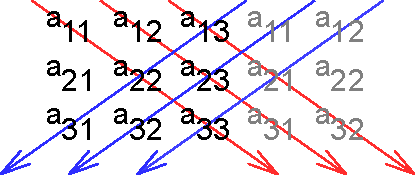
\includegraphics[width=0.35\textwidth]{Sarrus_rule.pdf}
    \caption{Reguła Sarrusa, źródło: Wikipedia.}
\end{figure}

\begin{fact}
    Objętość równoległościanu rozpiętego przez wektory będące wierszami (lub kolumnami) macierzy $A_{3\times 3}$ jest równa wartości bezwzględnej wyznacznika tej macierzy.
\end{fact}

\begin{theorem}[Cauchy'ego]
    \label{t:det is multiplicative}
    Dla dowolnych macierzy $A, B \in M_{n\times n}(\KK)$ zachodzi
    \[ \det(A\cdot B) = \det A \cdot \det B. \]
\end{theorem}
\begin{proof}
    TODO
\end{proof}

\begin{definition}
    Minor stopnia $k$ macierzy $A_{m\times n}$ to wyznacznik podmacierzy kwadratowej $k\times k$ powstałej przez wykreślenie $n-k$ kolumn oraz $m-k$ wierszy.
\end{definition}

Jeśli $A_{n\times n}$ jest macierzą kadratową, to wyznacznik macierzy powstałej przez wykreślenie $i$-tego wiersza i $j$-tej kolumny nazywamy \vocab{minorem odpowiadającym} elementowi $a_{ij}$ macierzy $A$ i oznaczamy $M_{ij}$.

\begin{definition}
    Dopełnienie algebraiczne elementu $a_{ij}$ macierzy kwadratowej $A = [a_{ij}]_{m\times n}$ to skalar
    \[ A_{ij} = (-1)^{i+j}M_{ij}. \]
\end{definition}

\begin{theorem}[Laplace'a]
    \label{t:Laplace}
    Niech $A = [a_{ij}]_{n\times n}$ będzie macierzą kwadratową. Wtedy dla każdego $i \in \{1,2\ldots,n\}$ 
    \[ \det A = \sum_{j=1}^n a_{ij}A_{ij}. \]
\end{theorem}

\begin{corollary}
    \label{c:determinant in triangular matrix}
    Wyznacznik macierzy trójkątnej jest równy iloczynowi elementów na jej przekątnej.
\end{corollary}